%%%%%%%%%%%%%%%%%%%%%%%%%%%%%%%%%%
%                                %
%    CONFIG FILE FOR TWISTYTEX   %
%          BY  KUHHIRTE          %
%                                %
%%%%%%%%%%%%%%%%%%%%%%%%%%%%%%%%%%
%
% SUPPORTED LANGUAGES:
%  ENG   ENGLISH
%  DEU   GERMAN
%

\newcommand{\lang}{DEU}

%
% ENTER THE TITLE AND THE AUTHOR
%

\newcommand{\thetitle}{Twisty Puzzles}
\newcommand{\theauthor}{kuhhirte}

%
% CUSTOM PREFACE:
% PROVIDE A CUSTOM PREFACE OR DELETE
% THE STANDARD PREFACE VIA UNCOMMENTING
%
%\newcommand{\chapterPrefaceContent}{}
\documentclass[12pt]{article}

\usepackage{fullpage} % less whitespace
\usepackage[utf8]{inputenc} % write ümläüts
\usepackage[T1]{fontenc} % output ümläuts
\usepackage{lmodern} % used font

\usepackage{ifthen}
\ifthenelse{\equal{\lang}{DEU}}{\usepackage[naustrian]{babel} % looks like austrian (post 1996)

% CHAPTERS

\newcommand{\chapterPreface}%
{Vorwort}
\newcommand{\chapterPrefaceContent}%
{Dieses Dokument wurde via der Skripte von \href{https://github.com/kuhhirte/twistytex}{kuhhirte/twistytex auf GitHub} erstellt.}

\newcommand{\textName}{Name}
\newcommand{\textShape}{Form}
\newcommand{\textBrand}{Marke}
\newcommand{\textMechanism}{Mechanismus}
\newcommand{\textComment}{Kommentar}

\newcommand{\textNoImage}{kein Bild vorhanden}}{}%
\ifthenelse{\equal{\lang}{ENG}}{\usepackage[british]{babel} % looks like british

% CHAPTERS

\newcommand{\chapterPreface}%
{Preface}
\newcommand{\chapterPrefaceContent}%
{This document was created using the structure and scripts from \href{https://github.com/kuhhirte/twistytex}{kuhhirte/twistytex on GitHub}.}

\newcommand{\textName}{Name}
\newcommand{\textShape}{Shape}
\newcommand{\textBrand}{Brand}
\newcommand{\textMechanism}{Mechanism}
\newcommand{\textComment}{Comment}

\newcommand{\textNoImage}{no image found}}{}%

\usepackage{csquotes} % quotation symbols 
\usepackage[babel=true]{microtype} % sexy micro typesetting
\usepackage[backend=biber,style=numeric]{biblatex} % bibliography package
\addbibresource{main.bib} % bibliogryphy style

\usepackage{tikz}

\usepackage{caption} % customizing captions of floating environments
\usepackage{gensymb} % general symbols (like degree)
\usepackage{wasysym} % extra general symbols
\usepackage{fontawesome}
\usepackage{graphicx}

\usepackage{hyperref} % create URLs and clickable refs
\usepackage{titling} % custom titling

\title{\thetitle}
\author{\theauthor}
\date{\today}

\newcommand{\cube}[6]%
{\begin{figure}[!htbp]%
		\begin{minipage}[t]{0.6\textwidth}%
			\begin{tabular}[t]{@{}ll@{}}%
				\textbf{\textName} & #1\\%
				\ifthenelse{\equal{\sortby}{Shape}}{}{\textbf{\textShape}&#2\\}%
				\ifthenelse{\equal{\sortby}{Brand}}{}{\textbf{\textBrand}&#3\\}%
				\ifthenelse{\equal{\sortby}{Mechanism}}{}{\textbf{\textMechanism}& #4}%
			\end{tabular}%
			
			\textbf{\textComment}%
			
			#6%
		\end{minipage}%
		\hfill%
		\begin{minipage}[t]{0.38\textwidth}%
			\IfFileExists{script/TEMPpictures/#5}%
			{\strut\vspace*{-\baselineskip}\newline\includegraphics[width=\textwidth]{script/TEMPpictures/#5}}%
			{\noindent\fbox{\begin{minipage}[t][7\baselineskip][t]{.95\textwidth}\centering \scriptsize\textNoImage\\\definecolor{lgrey}{RGB}{211,211,211}%
\definecolor{mgrey}{RGB}{127,127,127}%
\definecolor{dgrey}{RGB}{43,43,43}%
\definecolor{black}{RGB}{0,0,0}%
\tikz{\begin{tikzpicture}[y=.5, x=.5]
	%
	% UP FACE
	%
	% UP BACK LEFT
	\path[fill=lgrey] (77.3160,179.8000) -- (58.3520,171.7450)	-- (84.0160,165.3750) -- (102.560,174.7050) -- cycle;
	% UP BACK
	\path[fill=lgrey] (105.6080,173.9100) -- (87.3180,164.9820) -- (117.8550,157.5920) -- (135.5020,167.6260) -- cycle;
	% UP BACK RIGHT
	\path[fill=lgrey] (139.2460,167.0000) -- (122.0000,157.0690) -- (153.9800,149.2890) -- (170.2000,160.1090) -- cycle;
	% UP LEFT
	\path[fill=lgrey] (55.6290,170.6260) -- (33.7000,161.1960) -- (60.1690,154.0000) -- (81.5000,164.5300) -- cycle;
	% UP
	\path[fill=lgrey] (85.2200,164.0000) -- (64.2200,153.3090)	-- (95.2660,145.000) -- (115.8000,156.6790) -- cycle;
	% UP RIGHT
	\path[fill=lgrey] (119.9960,156.0000) -- (100.0000,144.1140) -- (132.7040,135.2000) -- (152.0000,148.1920) -- cycle;
	% UP FRONT LEFT
	\path[fill=lgrey] (30.0120,159.7000) -- (4.5000,148.6610) -- (32.3520,140.4000) -- (56.8000,152.6710) -- cycle;
	% UP FRONT
	\path[fill=lgrey] (60.6580,151.4000) -- (37.0000,139.5980) -- (68.4200,130.0000) -- (92.0000,143.4090) -- cycle;
	% UP FRONT RIGHT
	\path[fill=lgrey] (96.7130,142.3000) -- (73.5000,128.8870) -- (107.6730,118.5000) -- (129.9000,133.4910) -- cycle;
	%
	% FRONT FACE
	%
	% FRONT UP LEFT
	\path[fill=mgrey] (2.0000,145.5000) -- (5.5000,112.0000) -- (34.0000,102.0000) -- (31.0000,137.0000) -- cycle;
	% FRONT UP
	\path[fill=mgrey] (34.0000,136.5000) -- (37.0000,100.5000) -- (68.0000,89.5000) -- (67.0000,127.5000) -- cycle;
	% FRONT UP RIGHT
	\path[fill=mgrey] (70.5000,125.5000) -- (71.5000,88.0000) -- (107.0000,76.0000) -- (107.0000,115.0000) -- cycle;
	% FRONT LEFT
	\path[fill=mgrey] (6.0000,107.5000) -- (9.5000,76.5000) -- (36.5000,65.5000) -- (34.0000,98.0000) -- cycle;
	% FRONT
	\path[fill=mgrey] (37.0000,97.0000) -- (39.0000,64.0000) -- (69.0000,52.0000) -- (68.0000,85.0000) -- cycle;
	% FRONT RIGHT
	\path[fill=mgrey] (71.5000,84.0000) -- (72.0000,50.0000) -- (106.0000,36.0000) -- (106.5000,71.5000) -- cycle;
	% FRONT DOWN LEFT
	\path[fill=mgrey] (10.0000,72.5000) -- (13.0000,47.0000) -- (39.0000,34.5000) -- (37.0000,62.0000) -- cycle;
	% FRONT DOWN
	\path[fill=mgrey] (39.5000,61.0000) -- (41.0000,33.5000) -- (69.5000,20.0000) -- (69.0000,49.0000) -- cycle;
	% FRONT DOWN RIGHT
	\path[fill=mgrey] (72.0000,47.0000) -- (73.0000,18.0000) -- (105.5000,3.0000) -- (106.0000,33.5000) -- cycle;
	%
	% RIGHT FACE
	%
	% RIGHT UP FRONT
	\path[fill=dgrey] (133.3000,130.0000) -- (111.7870,114.6770) -- (111.0290,77.6020) -- (132.0090,94.5200) -- cycle;
	% RIGHT UP
	\path[fill=dgrey] (153.2000,144.2380) -- (136.0140,131.9620) -- (134.6240,96.8480) -- (151.3690,109.9880) -- cycle;
	% RIGHT UP BACK
	\path[fill=dgrey] (172.5000,158.0000) -- (156.4000,146.7090) -- (153.9570,112.0290) -- (168.9770,124.3890) -- cycle;
	% RIGHT FRONT
	\path[fill=dgrey] (131.8000,89.0000) -- (110.8850,71.2450) -- (110.2910,38.1120) -- (131.0210,58.0770) -- cycle;
	% RIGHT
	\path[fill=dgrey] (151.0000,105.1200) -- (134.5140,91.3600) -- (133.3140,60.1450) -- (149.2300,75.5250) -- cycle;
	% RIGHT BACK
	\path[fill=dgrey] (168.5500,120.0000) -- (153.4000,107.2330) -- (151.0600,77.3910) -- (165.2030,91.0410) -- cycle;
	% RIGHT DOWN FRONT
	\path[fill=dgrey] (130.6000,53.5000) -- (110.1900,32.9900) -- (109.5950,4.5300) -- (129.8650,26.3900) -- cycle;
	% RIGHT DOWN
	\path[fill=dgrey] (149.0000,71.8000) -- (133.1560,56.0770) -- (132.1800,28.8600) -- (147.2560,45.3680) -- cycle;
	% RIGHT DOWN BACK
	\path[fill=dgrey] (164.8000,87.3000) -- (150.7680,73.6490) -- (149.1200,47.2990) -- (161.9240,61.1590) -- cycle;
	% 
	% START OUTLINE
	% 
	\path[fill=black]
	(11.9580,47.0760) -- (0.0000,148.2560) -- (77.2300,179.9930) --
	(174.0700,160.6970) -- (162.8970,60.5650) -- (106.6070,0.0000) --
	cycle(104.8280,32.7830) -- (73.2260,45.7030) -- (73.8260,18.8710) --
	(104.6140,4.1910) -- cycle(129.6210,26.4930) -- (130.5000,53.0000) --
	(110.4400,32.8850) -- (109.8620,5.1820) -- cycle(68.0110,48.1230) --
	(40.3800,59.6200) -- (42.0750,34.2970) -- (68.6610,21.3970) --
	cycle(147.0210,45.4700) -- (148.6810,71.2760) -- (133.4110,55.9700) --
	(132.4610,29.5300) -- cycle(35.9100,61.3540) -- (11.3150,71.5800) --
	(14.0730,47.4400) -- (38.0250,36.0480) -- cycle(105.4100,70.7880) --
	(72.4800,82.8480) -- (73.1760,51.1210) -- (104.9460,37.8810) --
	cycle(130.7750,58.1880) -- (131.6820,88.6640) -- (111.1340,71.1280) --
	(110.5540,38.7110) -- cycle(164.6930,87.0000) -- (151.0130,73.5380) --
	(149.4130,47.9880) -- (161.6830,61.2760) -- cycle(66.9230,84.5800) --
	(37.9560,95.3630) -- (40.0310,65.1430) -- (68.0510,53.3360) --
	cycle(148.9870,75.6360) -- (150.7400,104.8290) -- (134.7600,91.2390) --
	(133.5880,60.7490) -- cycle(32.9700,97.0480) -- (7.2060,106.0450) --
	(10.4440,77.3500) -- (35.5540,66.9800) -- cycle(106.0000,114.2280) --
	(71.4900,124.5820) -- (72.4380,88.9840) -- (105.5360,77.2380) --
	cycle(131.7680,94.6440) -- (132.9530,129.6140) -- (112.0360,114.5440) --
	(111.2920,78.1340) -- cycle(164.9640,91.1510) -- (168.2190,119.6110) --
	(153.6390,107.1110) -- (151.3590,78.0310) -- cycle(66.1960,125.9710) --
	(35.0710,135.4410) -- (37.5410,101.4110) -- (67.0510,90.9710) --
	cycle(151.1260,110.1210) -- (153.1440,144.0410) -- (136.2570,131.8410) --
	(134.8940,97.3910) -- cycle(29.8840,136.6700) -- (3.0370,144.7200) --
	(6.4970,112.5100) -- (32.7330,103.1230) -- cycle(168.7400,124.5300) --
	(172.4100,157.8000) -- (156.6400,146.5800) -- (154.2480,112.6000) --
	cycle(128.6660,133.3930) -- (96.8360,141.7930) -- (74.4540,128.9690) --
	(107.6310,119.5190) -- cycle(90.8910,143.3260) -- (60.7710,151.0540) --
	(37.8610,139.6640) -- (68.4010,130.7900) -- cycle(151.2110,148.0860) --
	(120.1210,155.3620) -- (100.9110,144.2080) -- (132.6610,135.9780) --
	cycle(55.6210,152.5940) -- (30.1210,159.1640) -- (5.8400,148.7100) --
	(32.3300,141.2070) -- cycle(114.7010,156.5940) -- (85.3310,163.4140) --
	(65.3310,153.3910) -- (95.2310,145.7110) -- cycle(169.2800,160.0000) --
	(139.3800,166.4020) -- (123.2800,157.1720) -- (153.9400,149.9620) --
	cycle(80.2200,164.4500) -- (55.7300,170.2000) -- (34.8860,161.2560) --
	(60.1500,154.6390) -- cycle(134.3040,167.5240) -- (105.7280,173.5640) --
	(88.7580,165.0740) -- (117.8280,158.3640) -- cycle(101.1080,174.6140) --
	(77.4250,179.5740) -- (59.4550,171.8240) -- (83.9920,166.1440) -- cycle;
	\end{tikzpicture}}\end{minipage}}}
		\end{minipage}%
	\end{figure}%
}
\begin{document}

\begin{titlepage}
	\definecolor{yellow}{RGB}{255,255,127}%
\definecolor{white}{RGB}{255,255,255}%
\definecolor{blue}{RGB}{127,127,234}%
\definecolor{red}{RGB}{255,127,127}%
\definecolor{green}{RGB}{127,241,127}%
\definecolor{orange}{RGB}{255,220,127}%
\definecolor{gray}{RGB}{127,127,127}%
\tikz[remember picture,overlay] \node[inner sep=0pt] at (current page.center){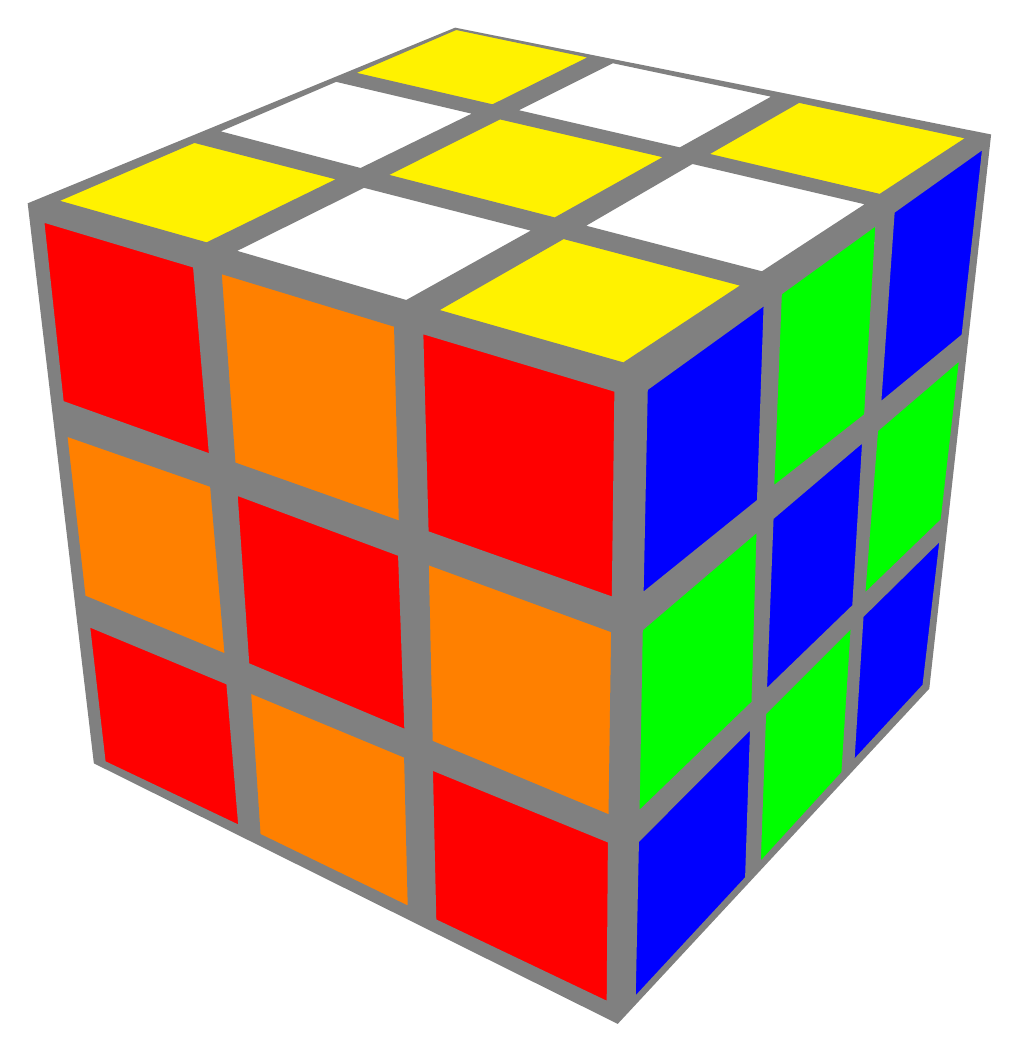
\begin{tikzpicture}[y=2, x=2]
	%
	% UP FACE
	%
	% UP BACK LEFT
	\path[fill=yellow] (77.3160,179.8000) -- (58.3520,171.7450)	-- (84.0160,165.3750) -- (102.560,174.7050) -- cycle;
	% UP BACK
	\path[fill=white] (105.6080,173.9100) --	(87.3180,164.9820) -- (117.8550,157.5920) -- (135.5020,167.6260) -- cycle;
	% UP BACK RIGHT
	\path[fill=yellow] (139.2460,167.0000) -- (122.0000,157.0690) -- (153.9800,149.2890) -- (170.2000,160.1090) -- cycle;
	% UP LEFT
	\path[fill=white] (55.6290,170.6260) -- (33.7000,161.1960) -- (60.1690,154.0000) -- (81.5000,164.5300) -- cycle;
	% UP
	\path[fill=yellow] (85.2200,164.0000) -- (64.2200,153.3090)	-- (95.2660,145.000) -- (115.8000,156.6790) -- cycle;
	% UP RIGHT
	\path[fill=white] (119.9960,156.0000) -- (100.0000,144.1140) -- (132.7040,135.2000) -- (152.0000,148.1920) -- cycle;
	% UP FRONT LEFT
	\path[fill=yellow] (30.0120,159.7000) -- (4.5000,148.6610) -- (32.3520,140.4000) -- (56.8000,152.6710) -- cycle;
	% UP FRONT
	\path[fill=white] (60.6580,151.4000) -- (37.0000,139.5980) -- (68.4200,130.0000) -- (92.0000,143.4090) -- cycle;
	% UP FRONT RIGHT
	\path[fill=yellow] (96.7130,142.3000) -- (73.5000,128.8870) -- (107.6730,118.5000) -- (129.9000,133.4910) -- cycle;
	%
	% FRONT FACE
	%
	% FRONT UP LEFT
	\path[fill=red] (2.0000,145.5000) -- (5.5000,112.0000) -- (34.0000,102.0000) -- (31.0000,137.0000) -- cycle;
	% FRONT UP
	\path[fill=orange] (34.0000,136.5000) -- (37.0000,100.5000) -- (68.0000,89.5000) -- (67.0000,127.5000) -- cycle;
	% FRONT UP RIGHT
	\path[fill=red] (70.5000,125.5000) -- (71.5000,88.0000) -- (107.0000,76.0000) -- (107.0000,115.0000) -- cycle;
	% FRONT LEFT
	\path[fill=orange] (6.0000,107.5000) -- (9.5000,76.5000) -- (36.5000,65.5000) -- (34.0000,98.0000) -- cycle;
	% FRONT
	\path[fill=red] (37.0000,97.0000) -- (39.0000,64.0000) -- (69.0000,52.0000) -- (68.0000,85.0000) -- cycle;
	% FRONT RIGHT
	\path[fill=orange] (71.5000,84.0000) -- (72.0000,50.0000) -- (106.0000,36.0000) -- (106.5000,71.5000) -- cycle;
	% FRONT DOWN LEFT
	\path[fill=red] (10.0000,72.5000) -- (13.0000,47.0000) -- (39.0000,34.5000) -- (37.0000,62.0000) -- cycle;
	% FRONT DOWN
	\path[fill=orange] (39.5000,61.0000) -- (41.0000,33.5000) -- (69.5000,20.0000) -- (69.0000,49.0000) -- cycle;
	% FRONT DOWN RIGHT
	\path[fill=red] (72.0000,47.0000) -- (73.0000,18.0000) -- (105.5000,3.0000) -- (106.0000,33.5000) -- cycle;
	%
	% RIGHT FACE
	%
	% RIGHT UP FRONT
	\path[fill=blue] (133.3000,130.0000) -- (111.7870,114.6770) -- (111.0290,77.6020) -- (132.0090,94.5200) -- cycle;
	% RIGHT UP
	\path[fill=green] (153.2000,144.2380) -- (136.0140,131.9620) -- (134.6240,96.8480) -- (151.3690,109.9880) -- cycle;
	% RIGHT UP BACK
	\path[fill=blue] (172.5000,158.0000) -- (156.4000,146.7090) -- (153.9570,112.0290) -- (168.9770,124.3890) -- cycle;
	% RIGHT FRONT
	\path[fill=green] (131.8000,89.0000) -- (110.8850,71.2450) -- (110.2910,38.1120) -- (131.0210,58.0770) -- cycle;
	% RIGHT
	\path[fill=blue] (151.0000,105.1200) -- (134.5140,91.3600) -- (133.3140,60.1450) -- (149.2300,75.5250) -- cycle;
	% RIGHT BACK
	\path[fill=green] (168.5500,120.0000) -- (153.4000,107.2330) -- (151.0600,77.3910) -- (165.2030,91.0410) -- cycle;
	% RIGHT DOWN FRONT
	\path[fill=blue] (130.6000,53.5000) -- (110.1900,32.9900) -- (109.5950,4.5300) -- (129.8650,26.3900) -- cycle;
	% RIGHT DOWN
	\path[fill=green] (149.0000,71.8000) -- (133.1560,56.0770) -- (132.1800,28.8600) -- (147.2560,45.3680) -- cycle;
	% RIGHT DOWN BACK
	\path[fill=blue] (164.8000,87.3000) -- (150.7680,73.6490) -- (149.1200,47.2990) -- (161.9240,61.1590) -- cycle;
	% 
	% START OUTLINE
	% 
	\path[fill=gray]
	(11.9580,47.0760) -- (0.0000,148.2560) -- (77.2300,179.9930) --
	(174.0700,160.6970) -- (162.8970,60.5650) -- (106.6070,0.0000) --
	cycle(104.8280,32.7830) -- (73.2260,45.7030) -- (73.8260,18.8710) --
	(104.6140,4.1910) -- cycle(129.6210,26.4930) -- (130.5000,53.0000) --
	(110.4400,32.8850) -- (109.8620,5.1820) -- cycle(68.0110,48.1230) --
	(40.3800,59.6200) -- (42.0750,34.2970) -- (68.6610,21.3970) --
	cycle(147.0210,45.4700) -- (148.6810,71.2760) -- (133.4110,55.9700) --
	(132.4610,29.5300) -- cycle(35.9100,61.3540) -- (11.3150,71.5800) --
	(14.0730,47.4400) -- (38.0250,36.0480) -- cycle(105.4100,70.7880) --
	(72.4800,82.8480) -- (73.1760,51.1210) -- (104.9460,37.8810) --
	cycle(130.7750,58.1880) -- (131.6820,88.6640) -- (111.1340,71.1280) --
	(110.5540,38.7110) -- cycle(164.6930,87.0000) -- (151.0130,73.5380) --
	(149.4130,47.9880) -- (161.6830,61.2760) -- cycle(66.9230,84.5800) --
	(37.9560,95.3630) -- (40.0310,65.1430) -- (68.0510,53.3360) --
	cycle(148.9870,75.6360) -- (150.7400,104.8290) -- (134.7600,91.2390) --
	(133.5880,60.7490) -- cycle(32.9700,97.0480) -- (7.2060,106.0450) --
	(10.4440,77.3500) -- (35.5540,66.9800) -- cycle(106.0000,114.2280) --
	(71.4900,124.5820) -- (72.4380,88.9840) -- (105.5360,77.2380) --
	cycle(131.7680,94.6440) -- (132.9530,129.6140) -- (112.0360,114.5440) --
	(111.2920,78.1340) -- cycle(164.9640,91.1510) -- (168.2190,119.6110) --
	(153.6390,107.1110) -- (151.3590,78.0310) -- cycle(66.1960,125.9710) --
	(35.0710,135.4410) -- (37.5410,101.4110) -- (67.0510,90.9710) --
	cycle(151.1260,110.1210) -- (153.1440,144.0410) -- (136.2570,131.8410) --
	(134.8940,97.3910) -- cycle(29.8840,136.6700) -- (3.0370,144.7200) --
	(6.4970,112.5100) -- (32.7330,103.1230) -- cycle(168.7400,124.5300) --
	(172.4100,157.8000) -- (156.6400,146.5800) -- (154.2480,112.6000) --
	cycle(128.6660,133.3930) -- (96.8360,141.7930) -- (74.4540,128.9690) --
	(107.6310,119.5190) -- cycle(90.8910,143.3260) -- (60.7710,151.0540) --
	(37.8610,139.6640) -- (68.4010,130.7900) -- cycle(151.2110,148.0860) --
	(120.1210,155.3620) -- (100.9110,144.2080) -- (132.6610,135.9780) --
	cycle(55.6210,152.5940) -- (30.1210,159.1640) -- (5.8400,148.7100) --
	(32.3300,141.2070) -- cycle(114.7010,156.5940) -- (85.3310,163.4140) --
	(65.3310,153.3910) -- (95.2310,145.7110) -- cycle(169.2800,160.0000) --
	(139.3800,166.4020) -- (123.2800,157.1720) -- (153.9400,149.9620) --
	cycle(80.2200,164.4500) -- (55.7300,170.2000) -- (34.8860,161.2560) --
	(60.1500,154.6390) -- cycle(134.3040,167.5240) -- (105.7280,173.5640) --
	(88.7580,165.0740) -- (117.8280,158.3640) -- cycle(101.1080,174.6140) --
	(77.4250,179.5740) -- (59.4550,171.8240) -- (83.9920,166.1440) -- cycle;
	\end{tikzpicture}};
	\thispagestyle{empty}      % Remove page numbering on this page
	{\center
		{
			\LARGE\thetitle       % Print the title data as defined above
			\\[5mm]               % 5mm spacing
			\large\theauthor      % Print the author data as defined above
			\\[5mm]               % 5mm spacing
			\large\today          % Todays date
			\\[30mm]              % 3cm spacing
		}
	}
	
	\tableofcontents
	
	\section*{\chapterPreface}
	
	\chapterPrefaceContent
	
\end{titlepage}

\input{script/cubes.tex}

\nocite{*}
\printbibliography[heading=bibintoc]
\end{document}